\section{A corpus comparison of proof-writing methods}
\label{sec:profile}

The case studies explain how particular preservation arguments work.
An exploratory survey asks how written proof methods are distributed
across the wider collection. The baseline is Mathlib at the collection's
dependency revision. Its guidelines accommodate term and tactic proofs
\citep{MathlibStyle}, making it a concrete comparison library with an
established range of styles.

\subsection{Sampling, extraction, and units of comparison}

The sampling population contains 122,457 tracked modules strictly under
\src{lean/OAI/}. From their paths we selected the 800 lowest SHA-256 ranks
of a fixed seed followed by the path, before fetching their contents.
The retained population list, seed, and Git blob identifiers reproduce
membership. The baseline comprises all 8,070 mathematical modules under
\src{Mathlib/} at the pinned revision, excluding infrastructure roots and
umbrella files. The scanner extracts explicitly written, named
\src{theorem} and \src{lemma} bodies: 13,309 in the OpenAI sample and
186,751 in Mathlib. Definitions, instances, anonymous examples, and
declarations produced by macros are outside this unit.

Nested comments and strings are masked before locating declaration
boundaries and the proof assignment. Extracted bodies cover 99.98\%
and 99.28\% of detected named declarations, respectively; the remaining
declarations, principally equation-style forms, are logged separately.
Coverage here concerns detected source declarations. Validation uses
forty stratified source inspections and eleven boundary checks, including
\src{let} bindings in theorem types and inline scoped declarations.
The validation record retains the inspected spans and two initial
theorem-type binding errors, followed by their extraction fixes.
This cohort tests known forms and boundary behavior; estimating error on
unseen declarations would require a separate validation sample.

A feature is recorded once per body when a listed unqualified token
occurs. Local claims include \src{have}, \src{suffices}, \src{obtain}, and
\src{calc}; arithmetic and algebra include \src{omega}, \src{linarith},
\src{nlinarith}, \src{ring}, and related tactics. Restricted simplification
records \src{simp}, \src{simpa}, or \src{simp_all} followed by \src{only}.
The retained script lists every token family. These indicators describe
written proof features. Elaborated traces would additionally identify
executed tactic nodes and their goal states.

Two summaries answer different questions. If module $m$ has $n_m$
extracted bodies and feature $f$ occurs in $c_{mf}$ of them, the pooled
rate is $\sum_m c_{mf}/\sum_m n_m$. The module-balanced rate is
$M^{-1}\sum_m c_{mf}/n_m$, over the $M$ modules with at least one
extracted body. Equivalently, select a proof-bearing module uniformly,
then select one of its bodies uniformly. There are 784 and 7,348 such
modules in the two corpora. We added module balancing after observing
certificate concentration; both summaries are retained as exploratory
analyses. The intervals in Table~\ref{tab:profile} resample the 784 OpenAI
modules using 1,500 percentile-bootstrap replicates. The 95\% intervals describe
sampling variation conditional on extraction and feature definitions,
with Mathlib treated as the retained census baseline.

\Needspace{27\baselineskip}
\begin{table}[H]
\centering
\caption{Module-balanced proof-body features (percent). The first three rows partition proof modes; subsequent features overlap. OpenAI intervals are exploratory 95\% module-bootstrap intervals. Mathlib is the census baseline at the pinned revision.}
\label{tab:profile}
\small
\setlength{\tabcolsep}{5pt}
\renewcommand{\arraystretch}{1.18}
\begin{tabular}{@{}p{6.7cm}rrr@{}}
\toprule
Written feature & OpenAI & Mathlib & OpenAI interval \\
\midrule
Outer tactic block & 92.8 & 54.5 & 91.8--93.9 \\[4pt]
Term with a tactic subproof & 0.5 & 5.7 & 0.2--0.9 \\[4pt]
Term without a tactic subproof & 6.7 & 39.8 & 5.7--7.7 \\[4pt]
\midrule
Rewrite or simplify & 72.5 & 52.4 & 70.3--74.6 \\[4pt]
Local claims or calculation chains & 61.1 & 21.0 & 58.8--63.6 \\[4pt]
Arithmetic or algebra tactics & 38.2 & 2.7 & 35.5--40.8 \\[4pt]
Restricted simplification & 38.5 & 13.0 & 36.4--40.9 \\[4pt]
Cases or induction & 19.8 & 12.8 & 18.0--21.8 \\[4pt]
Finite decision & 6.3 & 0.2 & 4.9--7.8 \\[4pt]
\bottomrule
\end{tabular}
\end{table}


\subsection{Separating subject composition, proof length, and method use}

In the full comparison, the largest difference concerns outer proof form:
the module-balanced share beginning in tactic mode is 92.8\% in the
OpenAI sample and 54.5\% in Mathlib. The former also has more bodies
containing local claims or calculation chains, arithmetic and algebra
tactics, and restricted simplification. In inspected case proofs these
features can work together: an intermediate claim records an estimate,
rewriting exposes scalar expressions, and \src{nlinarith} or \src{omega}
closes the resulting goal. The survey measures the prevalence of these
devices; source reading explains particular instances of their use.

Subject composition matters. Restricting to 18 shared top-level domains
retains 735 OpenAI proof-bearing modules, or 93.75\% of that sample.
Reweighting Mathlib's within-domain module averages to those OpenAI
domain shares gives tactic-mode rates of 93.0\% versus 63.8\%, local-claim
rates of 61.4\% versus 27.3\%, arithmetic rates of 37.6\% versus 7.1\%,
and restricted-simplification rates of 38.7\% versus 15.8\%.
Extensionality and congruence become similar: 13.8\% versus 13.1\%.
Directory labels provide a coarse subject control while retaining
different theorem populations and declaration roles.

Figure~\ref{fig:method-shift} expresses these contrasts as differences
from the Mathlib baseline in percentage points. The largest positive
differences concern tactic-mode proofs, local claims, and arithmetic
discharge. Term-only proofs are less frequent. Extensionality and
congruence sit close to the baseline after domain standardization,
showing that the difference is concentrated in particular proof devices.

\begin{figure}[H]
\centering
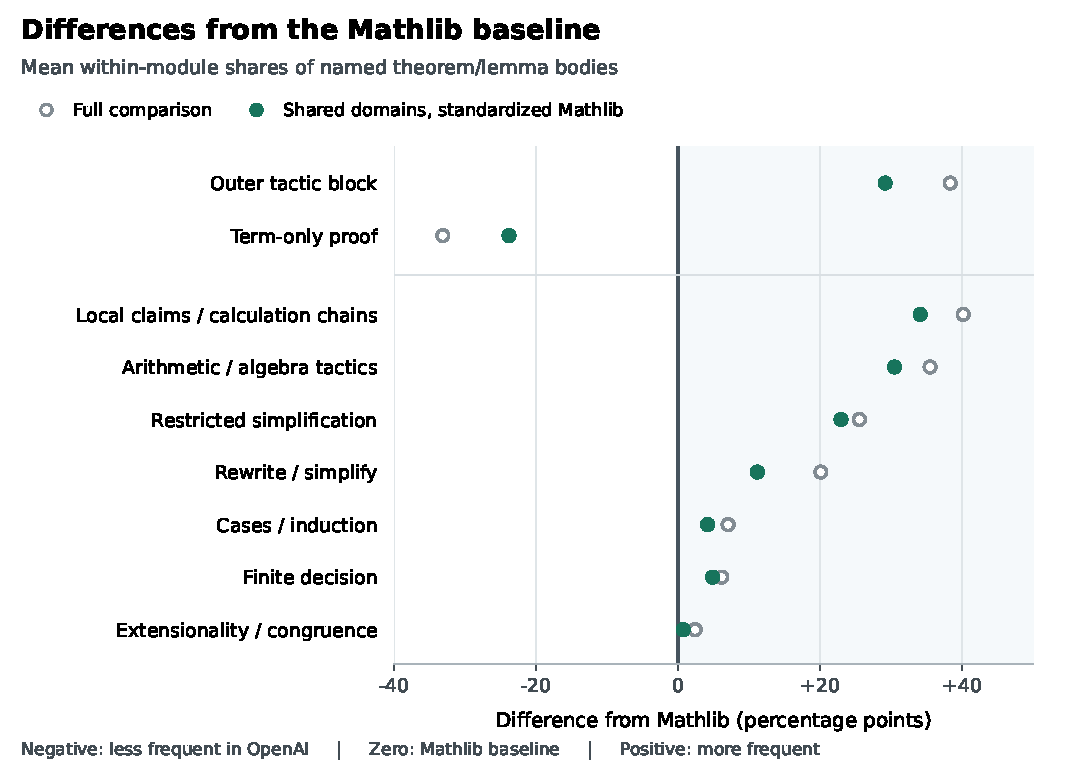
\includegraphics[width=\textwidth]{figures/method-shift.pdf}
\caption{OpenAI minus Mathlib differences in written proof-feature
prevalence, in percentage points. Zero denotes equal prevalence;
positive values indicate greater prevalence in the OpenAI sample.
Hollow markers compare all proof-bearing modules (784 OpenAI and
7,348 Mathlib). Green markers retain 735 OpenAI modules in 18 shared
domains and reweight Mathlib to the OpenAI domain shares. Both markers
lie at the same height for each feature and denote separate estimates
of the difference from Mathlib. Both comparisons average within-module
proof-body shares; features overlap except for the proof-mode
categories. The figure shows point estimates. Table~\ref{tab:profile}
reports absolute rates and 95\% OpenAI sampling intervals for selected
features in the full comparison. Table~\ref{tab:joint-profile} adds joint
subject and proof-length standardization.}
\label{fig:method-shift}
\end{figure}


Proof length changes the interpretation further. We jointly stratify by
the shared directory domains and four bands of nonempty body lines:
1--3, 4--10, 11--30, and 31 or more. The underlying measure remains
uniform selection of a proof-bearing module followed by a body within
it. Within a cell, a module's contribution is therefore proportional to
the fraction of its bodies in that cell. Mathlib's conditional feature
rates are reweighted to the OpenAI cell probabilities. This preserves
the module/body interpretation of Table~\ref{tab:profile}. The 69 shared
cells cover 93.75\% of that OpenAI measure.

For a feature $f$, write $\mu_C(f\mid s)$ for its conditional probability
in cell $s$ under corpus $C$, and let $w_s$ be the OpenAI cell probability
normalized over shared cells. The adjusted difference in percentage
points is
\[
  \Delta_f=100\sum_s w_s
  \bigl(\mu_{\mathrm{OpenAI}}(f\mid s)
       -\mu_{\mathrm{Mathlib}}(f\mid s)\bigr).
\]
Table~\ref{tab:joint-profile} compares this joint adjustment with the
subject-only results. Its exploratory intervals use 1,500 resamples of
OpenAI modules, recomputing their cell weights while keeping Mathlib's
cell means fixed.

\begin{table}[H]
\centering\small
\caption{OpenAI minus Mathlib differences in percentage points, with subject-only and joint subject/length standardization. Both use the module/body sampling measure. The 95\% percentile-bootstrap intervals resample OpenAI modules with Mathlib cell means fixed. The joint comparison covers 69 cells and 93.75\% of the OpenAI measure.}
\label{tab:joint-profile}
\setlength{\tabcolsep}{4pt}
\renewcommand{\arraystretch}{1.18}
\begin{tabular}{@{}p{6.0cm}rrr@{}}
\toprule
Written feature & Subject only & Subject + length & 95\% joint interval \\
\midrule
Outer tactic block & +29.2 & +10.4 & 9.3--11.5 \\[5pt]
Local claims or calculation chains & +34.1 & +5.8 & 4.4--7.3 \\[5pt]
Arithmetic or algebra tactics & +30.5 & +22.8 & 20.3--25.4 \\[5pt]
Restricted simplification & +22.9 & +7.7 & 5.4--9.8 \\[5pt]
Finite decision & +4.9 & +4.3 & 3.0--5.9 \\[5pt]
\bottomrule
\end{tabular}
\end{table}


Arithmetic and algebra tactics retain a difference of 22.8 percentage
points. The tactic-mode difference becomes 10.4 points and the
local-claim difference 5.8, compared with 29.2 and 34.1 under subject-only
adjustment. Thus proof-length composition is associated with much of
the latter contrasts. Length may itself reflect how an argument is
written, so conditioning on it changes the descriptive question.
The two comparisons show both the overall profile within subjects and
the remaining differences within broad subject/length cells.

Additional sensitivity checks remove each sampled directory-family group
in turn. The OpenAI arithmetic rate remains between 37.0\% and 38.7\%,
against 38.2\% in the full module-balanced sample. These groups are rough
proxies for developments; their exclusion shows that a single sampled
group does not account for the arithmetic profile. The retained data
also include the original pooled length-band comparison and alternative
family weights. Matching analogous mathematical tasks and declaration
roles would give a more specific baseline.

The listed general proof-search tokens, including \src{aesop},
\src{grind}, and \src{solve\_by\_elim}, have module-balanced rates of
0.07\% in the OpenAI sample and 3.35\% in Mathlib. Arithmetic tactics and simplification are themselves
automation, and other search tactics or imported macros can escape this
list. Similarly, \texttt{simp only} records explicit control of the rewrite
set. Its maintenance value depends on the surrounding proof. Mathlib's
guidance treats squeezing terminal simplification calls as a tradeoff
involving performance and fragility \citep{MathlibStyle}.

\subsection{Why certificate batches change the apparent distribution}

Concentration makes the distinction between modules and bodies essential.
Ten sampled OpenAI modules contribute 48.2\% of the extracted bodies;
the largest alone contributes 14.9\%. Consequently the pooled
finite-decision rate is 48.9\%, compared with the module-balanced 6.3\%.
Pooled rewrite/simplification rates are 41.5\% versus Mathlib's 48.8\%,
even though the module-balanced ordering in Table~\ref{tab:profile} is
reversed. Pooled rates describe the produced body population; module
averages describe practice under the module/body selection measure.

Reading these large files reveals an informative construction. The
sampled planar-packing module \src{LowBlock36\_10} contains 872 named
bodies, 792 of which contain a finite decision.\footnote{Source:
\href{https://github.com/openai/math/blob/fd4aeeb2ee4fc729c18d98444fed42fd0529eeeb/lean/OAI/Analysis/PlanarPacking/Certificate/LowBlock36_10.lean\#L16-L67}{\src{Analysis/PlanarPacking/Certificate/LowBlock36\_10.lean}, lines 16--67}.}
It defines exact integer interval data, checks individual entries with
\texttt{decide +kernel}, and assembles them into finite sums. A sampled
transonic barrier module chains Horner-step certificates with previously
proved tail bounds.\footnote{Source:
\href{https://github.com/openai/math/blob/fd4aeeb2ee4fc729c18d98444fed42fd0529eeeb/lean/OAI/MathematicalPhysics/Transonic/Certificates/Barrier59.lean\#L675-L678}{\src{MathematicalPhysics/Transonic/Certificates/Barrier59.lean}, lines 675--678}.}
The construction places exact data and small checks beneath soundness
and assembly lemmas. Lean 4.34.1 documents \texttt{decide +kernel} as
evaluating the decision instance by kernel reduction
\citep{LeanDecideSource}. This mechanism explains how a large collection
of short proofs serves as a numerical certificate for a later estimate.

The persistent arithmetic difference and the separate certificate layer
provide the clearest empirical findings. The larger unadjusted contrasts
also describe differences in proof form and length composition. Read
alongside the cases, these results motivate a division-of-work account:
preservation interfaces prepare mathematical obligations, and established
Lean devices check the resulting local steps. Section~\ref{sec:tactics-synthesis}
traces this interaction in particular proof bodies.
